\chapter{Overview}

\section{Genre}

2D Platform Fighting Game

\section{Theme}

When ordinary people come together, they can do extraordinary things.

\section{Philosophy}

\paragraph{} At the heart of OpenCombat lies its theme. The game's narrative is centered around combatants starting as normal entrants to the tournament and ends with them teaming up to defeat the business interests that seek to profit at the expense of society. The free and open source nature of the project allows the community to contribute to bug fixes, create mods and be part of testing future builds. Built into the game is the community management tool which seeks to bring people physically together to have shared experiences around OpenCombat.

\section{Value Proposition}

\paragraph{} OpenCombat offers many benefits to players as well as the community that surrounds them. Players can easily access the game and play it on any computer, making it a great choice for parties, small gatherings or personal play. Since it is built on a platform fighting game core, players will easily be able to jump in and engage with the experience even if they are never played it due to the accessibility of inputs. The open source nature of the game allows them to extend the experience as they see fit with mods and plugins they make themselves or acquire from the community. Tournament organizers of platform fighting games will appreciate the ability to easily obtain, install and modify any version of the game they wish. The community organizing tool also serves as a centralized spot for planning and hosting events which is ideal for players or TOs who organize gatherings.

\section{Goals}

\begin{enumerate}
    \item Design a community-driven game in which the experience in-play matters as much as the experience around-play.
    \item Develop an implementable crowdfunding model to decouple game development from venture capital.
    \item Experiment with cooperative open source development between a centralized team and the community.
\end{enumerate}

\section{Engine}

Godot Engine

\section{Technology Requirements}

\subsection{Platforms}

\begin{itemize}
    \item Windows (10+)
    \item macOS (10.15+)
    \item Linux via Snap
    \begin{description}
        \item[Note] Ubuntu is recommended when using the Snap package manager.
    \end{description}
\end{itemize}

\subsection{Minimum Specifications}

\paragraph{Note} The minimum specification for OpenCombat is based on surveys of consumers' hardware and software \autocite{valve_corporation_steam_nodate}. Components were selected based on their popularity and performance.

\subsubsection{CPU}

\begin{itemize}
    \item Intel or AMD CPUs are preferred.
    \item A minimum clock speed of 2.0 Ghz is required.
    \item A minimum of 2 cores is required.
\end{itemize}

\subsubsection{GPU}

\begin{itemize}
    \item The Intel HD Graphics 4000 is the minimum requirement.
    \item NVIDIA GeForce GTX 970 or newer is preferred.
    \item AMD Radeon RX 580 or newer is preferred.
\end{itemize}

\subsubsection{RAM}

\begin{itemize}
    \item 2 GBs of RAM is the minimum requirement.
    \item 4 GBs of RAM or more is recommended.
\end{itemize}

\pagebreak

\section{Distribution Methods}

\begin{itemize}
    \item Players can download a compiled executable from the website or the releases section of the GitHub repository.
    \item Players can compile their own version of the game from the Github repository.
    \item Players can install the game through their package managers on their respective platforms.
    \begin{description}
        \item [Windows] Chocolatey
        \item [macOS] Homebrew
        \item [Linux] Snap
    \end{description}
\end{itemize}

\section{Schedule}

\paragraph{Note} The following is a rough outline of all pre-release builds as well as what is included in the release. All versions prior to v1.0 are for testing and quality assurance.

\subsection{v0.1}

\subsubsection{Release Quarter}

Q4 2020

\subsubsection{Features}

\begin{itemize}
    \item Playable tutorial.
    \item Playable matches with customizable rules.
    \item Local and online matchmaking.
\end{itemize}

\subsection{v0.2}

\subsubsection{Release Quarter}

Q1 2021

\subsubsection{Features}

\begin{itemize}
    \item Complete character customization.
    \item Unlockable rewards.
\end{itemize}

\subsection{v1.0}

\subsubsection{Release Quarter}

Q3 2021

\subsubsection{Features}

\begin{itemize}
    \item Complete community organizing tool.
    \item Inclusion of official eSports rule-set.
\end{itemize}

\section{Marketplace Analysis}

\subsection{Target Audience}

\paragraph{} OpenCombat is designed for both casual and competitive players seeking an experience that is both accessible and easy to learn while also divergent and difficult to master. Based on the audience of other games in the genre, it is expected that the likely player base will be Millennials and younger generations who likely have their own laptops or average-performance desktops for school, work or personal use but may not have expensive gaming components. This group may exhibit some of the following characteristics:

\begin{itemize}
    \item They may be antisocial but they also do not mind having friends over or going to friends' homes to play games.
    \item They may have be more likely to pirate media since they likely cannot afford subscription services or prefer files for offline consumption.
    \item They may have no issues plugging their laptops into a TV and using it as a media station, gaming device, etc.
\end{itemize}

\subsection{Competitive Analysis}

\subsubsection{Super Smash Bros. Ultimate}

\paragraph{} Super Smash Bros. Ultimate is a 3D platform fighting game published by Nintendo and released on December 7th, 2018 globally. The player controls one of many characters from a variety of intellectual properties and uses their unique moves and attributes to knock their opponents outside of the arena \autocite{sakurai_super_2018}. It is the fifth game in the Super Smash Bros. franchise, the most recently of that franchise released and has sold over 17 million units  \autocite{nintendo_ir_nodate}.

\subparagraph{What Works Well}

\begin{itemize}
    \item The roster is mid-sized but has many characters from prominent franchises.
    \item Inputs to perform attacks are simple, intuitive and consistent across all characters.
    \item Rules are flexible allowing for both casual and competitive experiences.
    \item When mastered, movement is relatively fast and smooth.
    \item Plethora of additional modes that all utilize platform mechanics.
\end{itemize}

\subparagraph{What Could Be Improved}

\begin{itemize}
    \item Stages are too large which often results in difficulties knocking the opponents off of the stage even when they are at higher percentages.
    \item Although movement had been made faster from the two previous titles in the series, the lack of momentum in movement makes it difficult for characters to navigate platforms quickly.
    \item Although updates are free, additional downloadable characters and stages require purchasing.
\end{itemize}

\subsubsection{Super Smash Bros. Melee}

Super Smash Bros Melee is a 3D platform fighting game published by Nintendo and released on December 3rd, 2001 in the United States. The player controls one of many characters from a variety of intellectual properties owned by Nintendo and uses their unique moves and attributes to knock their opponents outside of the arena \autocite{sakurai_super_2001}. The game has been an active eSport since its release in the United States despite multiple sequels.

\subparagraph{What Works Well}

\begin{itemize}
    \item The roster is mid-sized but has many characters from prominent franchises.
    \item Inputs to perform attacks are simple, intuitive and consistent across all characters.
    \item Rules are flexible allowing for both casual and competitive experiences.
    \item When mastered, movement is relatively fast and smooth.
    \item Plethora of additional modes that all utilize platform mechanics.
\end{itemize}

\subparagraph{What Could Be Improved}

\begin{itemize}
    \item Stages are too large which often results in difficulties knocking the opponents off of the stage even when they are at higher percentages.
    \item The tech skill required to play this game at a competitive level is high and even dangerous to the health of players' hands \autocite{lee_haxs_2016}.
    \item Stage hazards cannot be turned off causing debate in the competitive community about which stages should be legal.
\end{itemize}

\begin{figure}[h!]
    \centering
    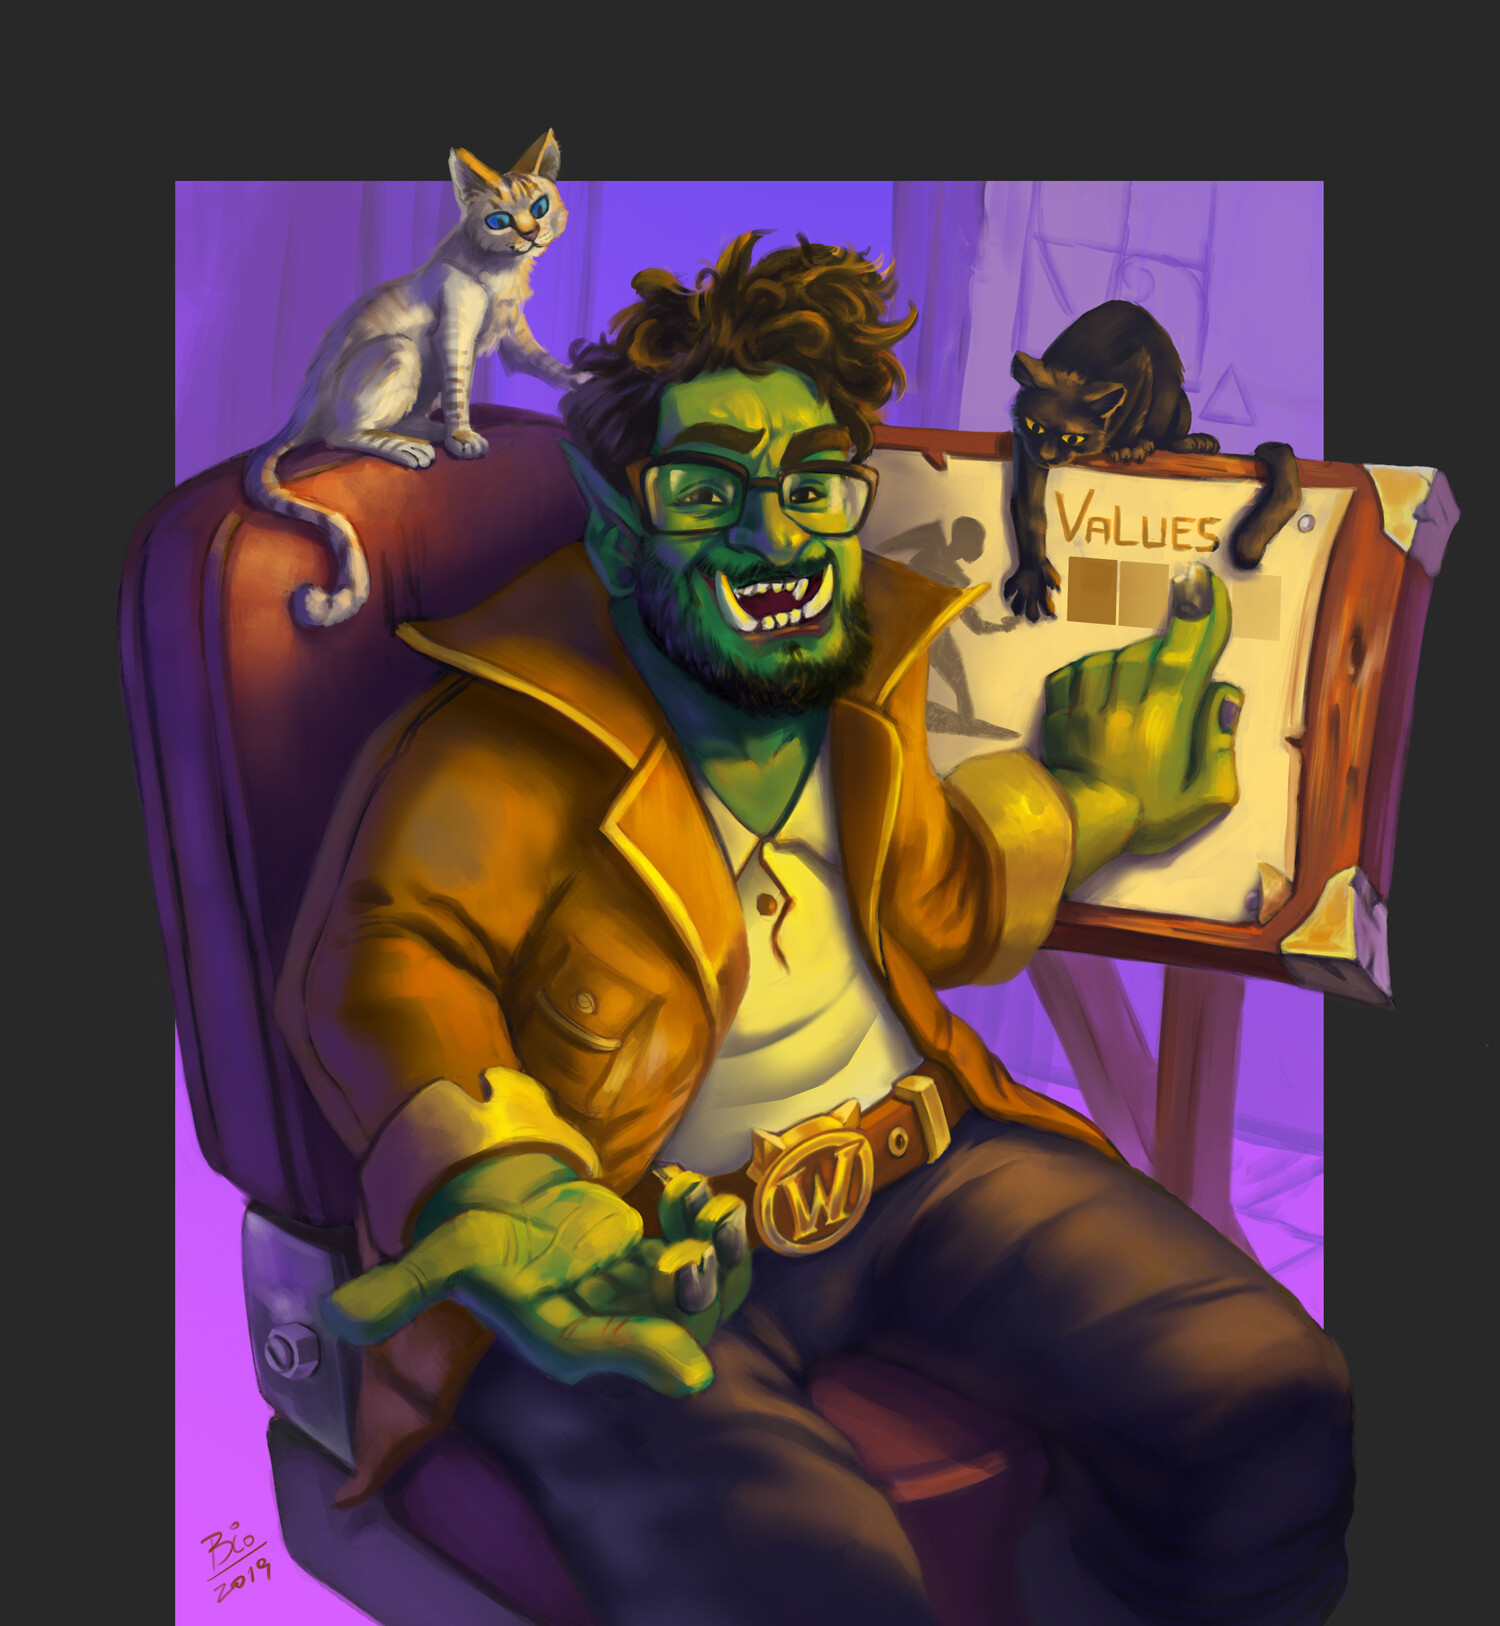
\includegraphics[width=0.4\linewidth]{images/characters-civilian.jpg}
    \caption{Cesar, The Mentor by Murillo Ribeiro. \nocite{ribeiro_cesar_2019}}
\end{figure}

\subsubsection{Rivals of Aether}

\paragraph{} Rivals of Aether is a 2D platform fighting game designed and developed by Dan Fornace. Similarly to the Super Smash Bros. franchise, the player controls one of many characters and uses their moves to knock the opponent out of the arena; unlike the Super Smash Bros. franchise, players cannot block their opponents' attacks or grab them. The game is currently an active eSport and has modding support through the Steam Workshop \autocite{fornace_rivals_2017}.

\subparagraph{What Works Well}

\begin{itemize}
    \item Inputs to perform attacks are simple, intuitive and consistent across all characters.
    \item When mastered, movement is relatively fast and smooth.
    \item Minimal lag on attacks and landing.
    \item The stages are unique enough to be different from one another but balanced enough to be used for competitive matches.
    \item Although the roster is small, each character feels unique.
\end{itemize}

\subparagraph{What Could Be Improved}

\begin{itemize}
    \item There no items or rule adjustments to play casually.
    \item Although updates are free, additional downloadable characters and stages require purchasing.
    \item Stages are too large which often results in slower matches.
\end{itemize}

\subsubsection{Brawlhalla}

\paragraph{} Brawlhalla is a 2D platform fighting game published by Ubisoft and released on October 17th, 2017. Similarly to other games in the genre, players pick from a variety of characters across intellectual properties as well as characters unique to the game and use their unique attributes and fighting styles to knock their opponents out of the arena \autocite{blue_mammoth_games_brawlhalla_2017}. The free-to-play nature of the game has made it accessible to most users and had over 8 million players with at least one achievement on Steam from the game as of 2018 \autocite{orland_valve_2018}.

\subparagraph{What Works Well}

\begin{itemize}
    \item Inputs to perform attacks are simple, intuitive and consistent across all characters.
    \item When mastered, movement is relatively fast and smooth.
    \item Minimal lag on attacks and landing.
    \item The stages are unique enough to be different from one another but balanced enough to be used for competitive matches.
\end{itemize}

\subparagraph{What Could Be Improved}

\begin{itemize}
    \item Although the game is free-to-play, various components of the game require in-game purchases.
    \item Stages are too large which often results in slower matches.
\end{itemize}